% ----------------------------------------------------------
\chapter{Systematic Review of the Literature: Text Regression}\label{ap:rsl_regression_law}
% ----------------------------------------------------------

In this SRL, we focused on finding papers related to the application of regression techniques on legal texts written in the Portuguese language. However, such a task did not succeed due to the lack of work in that matter. Thus, we applied a broader search regarding the application of regression in texts without context or language limitations.

\section{Definition of Search Questions}

The question of this search is: ``What are the regression techniques applied to texts considering any applications and languages?''

\section{Search Strategies}

The search used the following search string:

% TODO: Continue from here.
\begin{verbatim}
  ( "regression on text*"  OR  "text* regression"  OR  "regression text*"  
  OR  "regression from text*"  OR  "regression for text*" )  
  AND NOT  "logistic regression"  
\end{verbatim}



\section{Search Resources}
In this SRL, we searched on the following bases:

\begin{itemize}[noitemsep]
    \item Scopus
    \item ACM Digital Library
    \item IEEE Xplore
    \item Web of Science
\end{itemize}

\section{Selection Criteria}

Following the questions of this research, we defined a set of inclusion and exclusion criteria. The process of selection embraced the reading of title, abstract and keywords, and the accordance with the criteria.

The following is the list of inclusion criteria:

\begin{itemize}[noitemsep]
    \item Published in journal or conference
    \item Involves regression applied to textual data;
    \item Involves Machine Learning or Text Mining;
    \item The techniques used are named;
    \item Empirical Work;
    \item Published from 2010 and December 2020.
\end{itemize}

And the following is the list of exclusion criteria:

\begin{itemize}[noitemsep]
    \item Work not written in Portuguese or English;
    \item Published over 10 years ago;
    \item Does not involve regression applied to textual data;
    \item Does not involve Machine Learning or Text Mining;
    \item Theoretic work.
\end{itemize}

\section{Data Extraction}
In the SRL from this section, we focused on retrieving the text representation, the regression techniques used and the evaluation metrics.

\section{Search Execution and Preliminary Analysis}

After applying the first search string to the knowledge base on December 1, 2020 for researches published from 2010 to December 2020, the search returned 124 documents. After reading title, abstract and keywords and applying the selection criteria, the number of papers reduced to 18.


\section{Results and Discussion}

% Técnicas mais comuns

In this section, we show the results and analysis in terms of regression techniques applied to text. In this part of this research, we focused on the regression techniques applied in any domains. In Figure \ref{fig:rsl_regression_year_publishing}, one can notice the distribution by year of the research interest on the area of the regression applied to texts.

% Publicações por ano

\begin{figure}[htb]
    \centering
    \caption{Papers published by year}
    \label{fig:rsl_regression_year_publishing}
    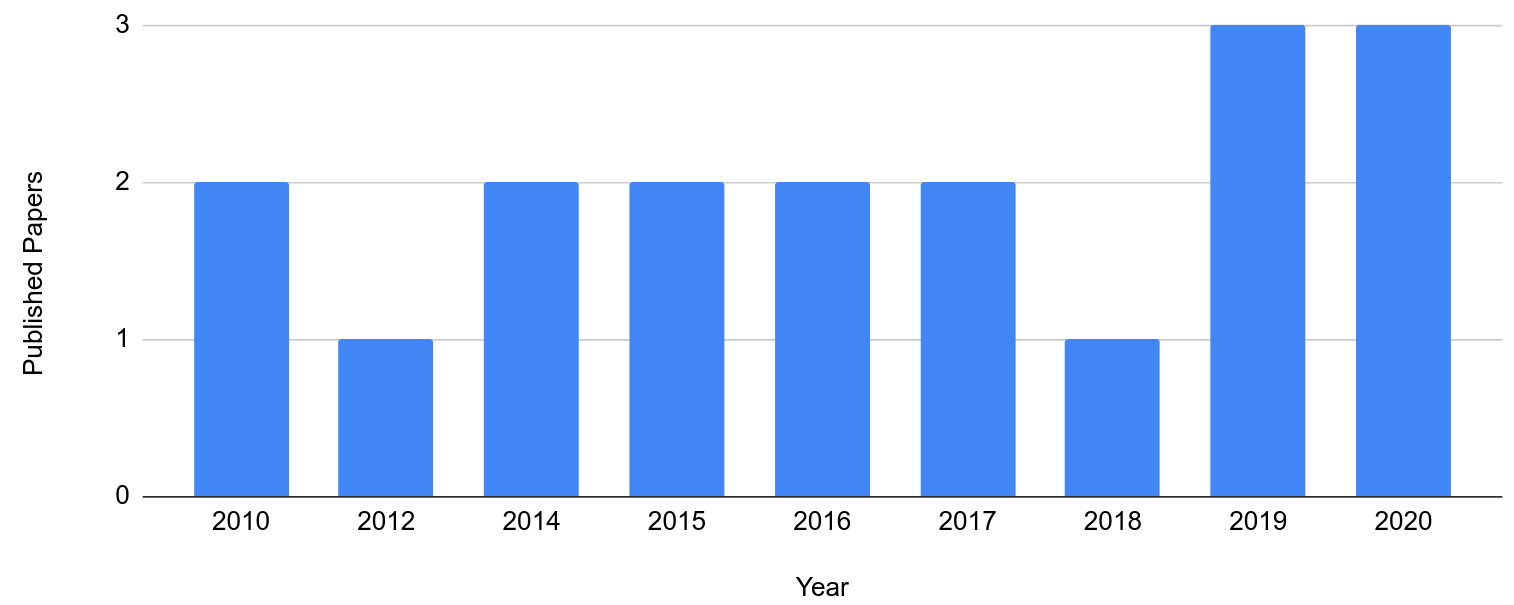
\includegraphics[width=\textwidth]{images/appendix/rsl_regression.png}
\end{figure}


In Table \ref{tab:rsl_regression_representation}, there are the representation techniques used in the selected work from the SRL. The most common technique is the Bag of Words followed by the N-Grams and TF-IDF, that is Vector Space Models representations. There is also neural based techniques such as word embeddings.


\begin{table}[htb]
\centering
\caption{Representation techniques in papers from regression SRL}
\label{tab:rsl_regression_representation}
\footnotesize
\begin{tabular}{@{}cc@{}}
\toprule
\textbf{Representation} & \textbf{Papers} \\ \midrule
Bag of Words & 8 \\
N-gram & 4 \\
TF-IDF & 4 \\
Metadata & 2 \\
Part-of-Speech Tag & 2 \\
Word Embeddings & 2 \\
Context ependence & 1 \\
Dependency relations & 1 \\
LDA & 1 \\
LSA & 1 \\ \bottomrule
\end{tabular}
\end{table}


In Table \ref{tab:rsl_regr_tech}, there are the most frequent regression techniques applied in the selected work. The most common is the Support Vector Machine, followed by Linear Regression, Convolution Neural Network, Elastic Net, Gaussian Copula, and Gradient Boosting.

\begin{table}[htb]
\centering
\caption{Regression techniques applied in the  papers from SRL}
\label{tab:rsl_regr_tech}
\footnotesize
\begin{tabular}{@{}lc@{}}
\toprule
\multicolumn{1}{c}{\textbf{Regression Tech}} & \textbf{Papers} \\ \midrule
Support Vector Machine & 7 \\
Linear Regression & 5 \\
Convolutional Neural Network & 2 \\
Elastic Net & 2 \\
Gaussian Copula & 2 \\
Gradient Boosting & 2 \\
Conditional Generative Adversarial Network & 1 \\
Gaussian Process & 1 \\
kNN & 1 \\
Lasso & 1 \\
Multinomial logistic text regression & 1 \\
Random Forest & 1 \\
Ridge & 1 \\
XGBoosting & 1 \\ \bottomrule
\end{tabular}
\end{table}

In Table \ref{tab:rsl_regr_evaluation}, there are the most common evaluation metrics for regression applied in the select work. One can note the Mean Absolute Error (MAE) is the most common, followed by Mean Square Error (MSE) and Root Mean Square Error (RMSE).

\begin{table}[htb]
\centering
\caption{Evaluation metrics for regression}
\label{tab:rsl_regr_evaluation}
\footnotesize
\begin{tabular}{@{}lc@{}}

\toprule
\multicolumn{1}{c}{\textbf{Evaluation Metric}} & \textbf{Papers} \\ \midrule
Mean Absolute Error & 9 \\
Mean Square Error & 3 \\
Root Mean Square Error & 3 \\
Pearson's correlation & 2 \\
Relative Absolute Error & 2 \\
Root Relative Squared Error & 2 \\
Adjusted R2 & 1 \\
F-variation & 1 \\
Kendall's Tau & 1 \\
R$^2$ & 1 \\
RAE & 1 \\
Spearman's Correlation & 1 \\
Standardization on Beta & 1 \\
Symmetric Mean Absolute Percentage Error & 1 \\
Value of $t$ & 1 \\ \bottomrule
\end{tabular}
\end{table}

